%!TEX root = ../../beamer.tex
\begin{frame}
\begin{center}
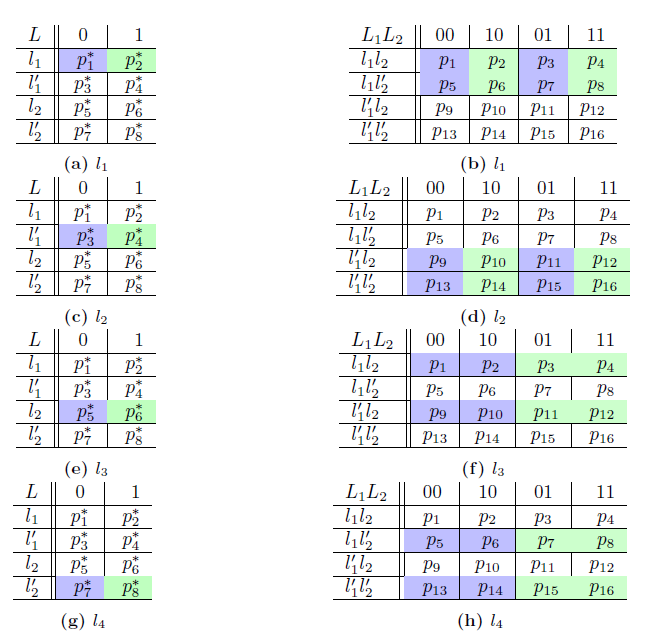
\includegraphics[width=0.6\textwidth]{fig/kccondexample.png}\\
\end{center}
% \begin{table}
% \centering
% %!TEX root = ../plos_template.tex
\begin{subtable}[t]{0.4\textwidth}
\centering
\begin{tabular}{ l || c | r }
	$L$  &	0 & 1\\ \hline
    $l_1$ & \cellcolor{DeepBlue!35} $p^*_1$ & \cellcolor{DeepRed!35} $p^*_2$\\ \hline
    $l'_1$ & $p^*_3$ & $p^*_4$\\ \hline
    $l_2$ & $p^*_5$ & $p^*_{6}$\\ \hline
    $l'_2$ & $p^*_{7}$ & $p^*_{8}$\\
    \hline
    \end{tabular}
    \caption{$l_1$}
    \label{tab:il1}
\end{subtable}
~~~~~~
\begin{subtable}[t]{0.4\textwidth}
\centering
	\begin{tabular}{ l || c | c | c | r }
	$L_1 L_2$  &	00 & 10 & 01 & 11\\ \hline
    $l_1 l_2$ & \cellcolor{DeepBlue!35} $p_1$ & \cellcolor{DeepRed!35} $p_2$ & \cellcolor{DeepBlue!35} $p_3$ & \cellcolor{DeepRed!35} $p_4$\\ \hline
    $l_1 l'_2$ & \cellcolor{DeepBlue!35} $p_5$ & \cellcolor{DeepRed!35} $p_6$ & \cellcolor{DeepBlue!35} $p_7$ & \cellcolor{DeepRed!35} $p_8$\\ \hline
    $l'_1 l_2$ & $p_9$ & $p_{10}$ & $p_{11}$ & $p_{12}$\\ \hline
    $l'_1 l'_2$ & $p_{13}$ & $p_{14}$ & $p_{15}$ & $p_{16}$\\
    \hline
	\end{tabular}
	\caption{$l_1$}
    \label{tab:dl1}
\end{subtable}

% \begin{subtable}[t]{0.4\textwidth}
\centering
\begin{tabular}{ l || c | r }
	$L$  &	0 & 1\\ \hline
    $l_1$ & $p^*_1$ & $p^*_2$\\ \hline
    $l'_1$ & \cellcolor{blue!25} $p^*_3$ & \cellcolor{green!25} $p^*_4$\\ \hline
    $l_2$ & $p^*_5$ & $p^*_{6}$\\ \hline
    $l'_2$ & $p^*_{7}$ & $p^*_{8}$\\    
    \hline
    \end{tabular}
    \caption{$l_2$}
    \label{tab:il2}
\end{subtable}
~~~~~~
\begin{subtable}[t]{0.4\textwidth}
\centering
	\begin{tabular}{ l || c | c | c | r }
	$L_1 L_2$  &	00 & 01 & 10 & 11\\ \hline
    $l_1 l_2$ & $p_1$ & $p_2$ & $p_3$ & $p_4$\\ \hline
    $l_1 l'_2$ & $p_5$ & $p_6$ & $p_7$ & $p_8$\\ \hline
    $l'_1 l_2$ & \cellcolor{blue!25} $p_9$ & \cellcolor{blue!25} $p_{10}$ & \cellcolor{green!25} $p_{11}$ & \cellcolor{green!25} $p_{12}$\\ \hline
    $l'_1 l'_2$ & \cellcolor{blue!25} $p_{13}$ & \cellcolor{blue!25} $p_{14}$ & \cellcolor{green!25} $p_{15}$ & \cellcolor{green!25} $p_{16}$\\
    \hline
	\end{tabular}
	\caption{$l_2$}
    \label{tab:dl2}
\end{subtable}
% %!TEX root = ../plos_template.tex
\begin{subtable}[t]{0.4\textwidth}
\centering
\begin{tabular}{ l || c | r }
	$L$  &	0 & 1\\ \hline
    $l_1$ & $p^*_1$ & $p^*_2$\\ \hline
    $l'_1$ & $p^*_3$ & $p^*_4$\\ \hline
    $l_2$ & \cellcolor{DeepBlue!35} $p^*_5$ & \cellcolor{DeepRed!35} $p^*_{6}$\\ \hline
    $l'_2$ & $p^*_{7}$ & $p^*_{8}$\\
    \hline
    \end{tabular}
    \caption{$l_3$}
    \label{tab:il3}
\end{subtable}
~~~~~~
\begin{subtable}[t]{0.4\textwidth}
\centering
	\begin{tabular}{ l || c | c | c | r }
	$L_1 L_2$  &	00 & 10 & 01 & 11\\ \hline
    $l_1 l_2$ & \cellcolor{DeepBlue!35} $p_1$ & \cellcolor{DeepBlue!35} $p_2$ & \cellcolor{DeepRed!35} $p_3$ & \cellcolor{DeepRed!35} $p_4$\\ \hline
    $l_1 l'_2$ &  $p_5$ & $p_6$ & $p_7$ & $p_8$\\ \hline
    $l'_1 l_2$ & \cellcolor{DeepBlue!35} $p_9$ & \cellcolor{DeepBlue!35} $p_{10}$ & \cellcolor{DeepRed!35} $p_{11}$ & \cellcolor{DeepRed!35} $p_{12}$\\ \hline
    $l'_1 l'_2$ & $p_{13}$ & $p_{14}$ & $p_{15}$ & $p_{16}$\\
    \hline
	\end{tabular}
	\caption{$l_3$}
    \label{tab:dl3}
\end{subtable}

% %!TEX root = ../plos_template.tex
\begin{subtable}[t]{0.4\textwidth}
\centering
\begin{tabular}{ l || c | r }
	$L$  &	0 & 1\\ \hline
    $l_1$ & $p^*_1$ & $p^*_2$\\ \hline
    $l'_1$ & $p^*_3$ & $p^*_4$\\ \hline
    $l_2$ & $p^*_5$ & $p^*_{6}$\\ \hline
    $l'_2$ & \cellcolor{DeepBlue!35} $p^*_{7}$ & \cellcolor{DeepRed!35} $p^*_{8}$\\
    \hline
    \end{tabular}
    \caption{$l_4$}
    \label{tab:il4}
\end{subtable}
~~~~~~
\begin{subtable}[t]{0.4\textwidth}
\centering
	\begin{tabular}{ l || c | c | c | r }
	$L_1 L_2$  &	00 & 10 & 01 & 11\\ \hline
    $l_1 l_2$ & $p_1$ & $p_2$ & $p_3$ & $p_4$\\ \hline
    $l_1 l'_2$ & \cellcolor{DeepBlue!35} $p_5$ & \cellcolor{DeepBlue!35} $p_6$ & \cellcolor{DeepRed!35} $p_7$ & \cellcolor{DeepRed!35} $p_8$\\ \hline
    $l'_1 l_2$ & $p_9$ & $p_{10}$ & $p_{11}$ & $p_{12}$\\ \hline
    $l'_1 l'_2$ & \cellcolor{DeepBlue!35} $p_{13}$ & \cellcolor{DeepBlue!35} $p_{14}$ & \cellcolor{DeepRed!35} $p_{15}$ & \cellcolor{DeepRed!35} $p_{16}$\\
    \hline
	\end{tabular}
	\caption{$l_4$}
    \label{tab:dl4}
\end{subtable}

% \caption{The sheaf condition for the two-locus-two phenotype value example. The left column represents \emph{atomic} probabilities that relate probabilities via equations \ref{eq:pparsys} from the empirical models given in the right hand column. Each row in all tables is required to sum to 1.}
% \label{tab:sheaf}
%\end{table}
\end{frame}
